\section{Thermodynamical analysis of possible defects}

First step of current investigation is the study of possible defects within LiFePO$_4$ structure. There are can be observed several types of defects:
\begin{enumerate} 
	\item Hydrogen in octahedral void sites of LFP;
	\item Hydrogen in tetrahedral void sites of LFP;
	\item Hydrogen interstitial defect with lithium vacancy;
	\item Hydrogen substitutional defect in place of Li and Fe vacancy sites;
	\item Hydrogen substitutional defect in place of P vacancy site without electronic compensation (4 of H);
	\item Hydrogen substitutional defect in place of P vacancy site with charge compensation (5 of H).
\end{enumerate}

The chemical potential of hydrogen is defined as:
\begin{equation}
    \mu(H)=\frac{1}{2}[\mu(H_2O_{gas})-\frac{1}{2}\mu(O_2)]
\end{equation}

According that, the chemical potential of hydrogen $\mu(H)$ is equal to -0.83 eV. Using that parameter and taking into account the value of oxygen chemical potential, which is equal to  -11.52 eV, the chemical potentials of iron, lithium and phosphorus can be calculated as:

\begin{eqnarray}
\label{FeLiP}
  &\mu(Fe)=\frac{1}{2}[\mu(Fe_2O_3)-\frac{3}{2}\mu(O_2)] \nonumber \\ 
  &\mu(Li)=\frac{1}{2}[\mu(Li_3PO_4)-\mu(LiFePO_4)+\mu(Fe)] \\
  &\mu(P)=\frac{1}{2}[\mu(LiFePO_4)-\mu(Li_3PO_4)-3\cdot\mu(Fe)-4\cdot\mu(O_2)] \nonumber
\end{eqnarray}

\begin{table}[h]
\caption{Chemical potentials}
\label{tabular:LiFeP}
\begin{center}
\begin{tabular}{|c|c|c|}
\hline
& &  \\
\textbf{Type of atom} & \textbf{My $\mu(atom)$} & \textbf{Previous $\mu(atom)$}  \\
\hline
& &  \\
Fe & -10.09eV & 1.40eV \\ 
\hline
& &  \\
Li &  -5.82eV  &  0.64eV \\ 
\hline
& &  \\
P &  -10.05eV & 3.46 eV \\ 
\hline
\end{tabular}
\end{center}
\end{table}

For -11.52eV chemical potential of oxygen the chemical potentials of different atoms above were found: -5.82eV for Li, -10.09eV for Fe and -10.05 for P. In order to discuss the mechanism of vacancy formation or interstitial/substitutional defect it is necessary to emphasize the charge compensation mechanism. In case of electron incorporation (extraction) to (from) ideal LiFePO$_4$ material the iron change its valence between Fe$^{2+}$ and Fe$^{3+}$. For evaluation the possibility of this behaviour the solution energies of several defect types have been observed and studied during this section.

\textbf{1. Interstitial hydrogen in octahedral void sites of ideal LFP}

During study of interstitial defects two configurations of hydrogen within empty octahedral voids of LFP structure were found.  After calculating the stable positions with minimum of energy were found and energies of defects existing are equal to:
\begin{enumerate}
	\item First initial position of hydrogen is within empty octahedral void of ideal LFP near the iron octahedral site with distance between Fe and H is around 1.95 \AA, which is changes after relaxation to 1.99 \AA. After relaxation the distance between hydrogen and the closest oxygen H-O$_1$ is change from 0.99 \AA to 1.04 \AA, the distance between hydrogen and second neihbour of oxygen H-O$_2$ changes from 2.1\AA to 1.55 \AA and hydrogen is located in bond between O$_1$ and O$_2$, creating the hydrogen bond, Fig.\ref{ris:oct1}. The formation energy of such defect is equal to -0.4667 eV.
	\item In the second case the hydrogen is located in the empty octahedral void near the phosphorus tetrahedral site with the distance between P and H is equal to 1.16 \AA: two empty tetrahedral voids and the iron octahedral are located near them. After relaxation the distance between the hydrogen and the neighboring oxygen H-O$_1$ decreases from 1.04 \AA to 1.01 \AA and the distance between the hydrogen and the second neighboring oxygen H-O$_2$ changes from 2.52 \AA to 1.84 \AA, Fig.\ref{ris:oct2}. The formation energy of such defect is equal to -0.596 eV.
\end{enumerate}

\begin{figure}[ht]
\begin{minipage}[ht]{0.49\linewidth}
\center{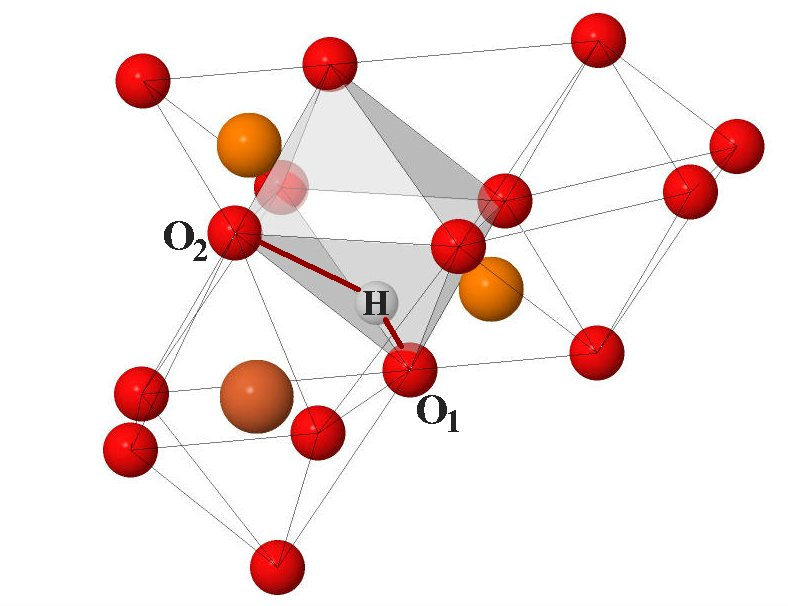
\includegraphics[width=0.9\linewidth]{pictures/oct1beforeCROP.png} \\ a)}
\end{minipage}
\hfill
\begin{minipage}[ht]{0.49\linewidth}
\center{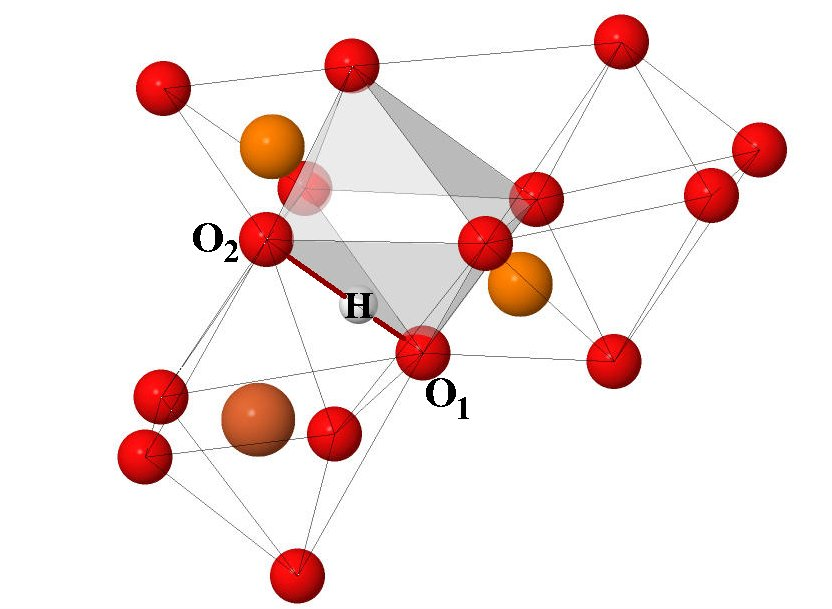
\includegraphics[width=0.9\linewidth]{pictures/oct1afterCROP.png} \\ b)}
\end{minipage}
\caption{Changes of hydrogen localization afret strucrural optimization in 1 case of octahedral void}
\label{ris:oct1}
\end{figure}

\begin{figure}[ht]
\begin{minipage}[h]{0.49\linewidth}
\center{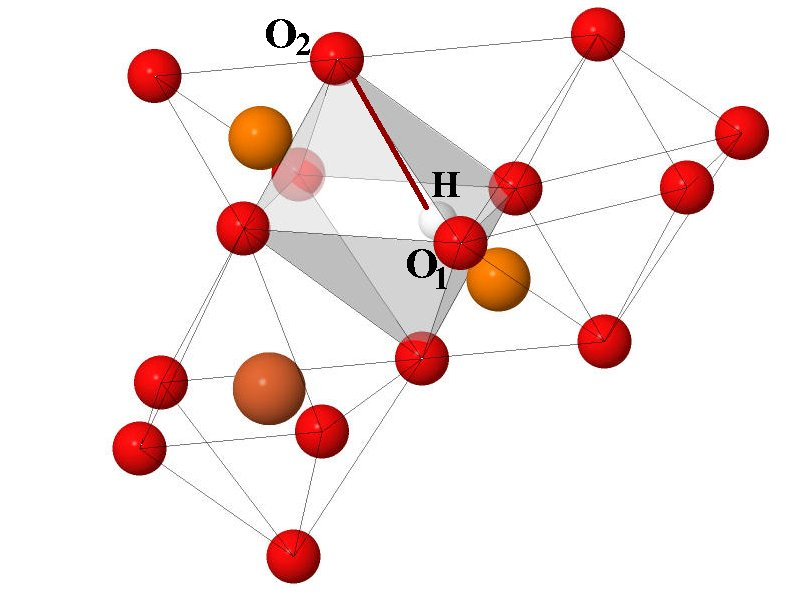
\includegraphics[width=0.9\linewidth]{pictures/oct2beforeCROP.png} \\ a)}
\end{minipage}
\hfill
\begin{minipage}[ht]{0.49\linewidth}
\center{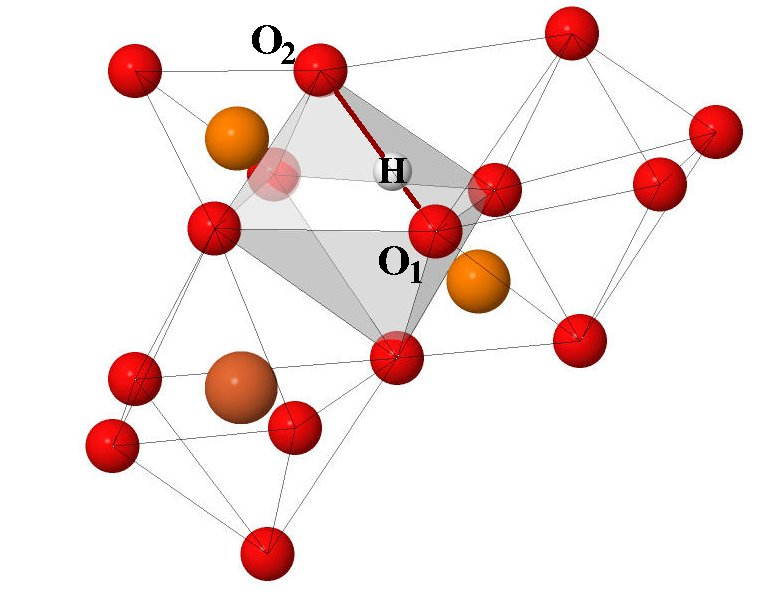
\includegraphics[width=0.9\linewidth]{pictures/oct2afterCROP.png} \\ b)}
\end{minipage}
\caption{Changes of hydrogen localization afret strucrural optimization in 2 case of octahedral void}
\label{ris:oct2}
\end{figure}


\textbf{2. Interstitial hydrogen in tetrahedral void sites of ideeal LFP}

During study of interstitial defects of hydrogen within LFP structure two different configuration of them were found. 
\begin{enumerate}
	\item The first type of hydrogen localization within empty tetrahedral void corresponds to configuration on Fig.\ref{ris:tet1}, where hydrogen locates in the middle of tetrahedral oxygen environment. After relaxation of all positions of atoms, distances between interstitial hydrogen and other atoms are changed: H-O$_1$ from 1.84 \AA to 2.54 \AA; H-O$_2$ from 1.69 \AA to 1.54 \AA; H-Fe from 2.09 \AA to 1.48 \AA. It is important to note the change of distance between O$_2$ atom and neighboring iron: it increases from 2.21 \AA to 2.98 \AA. The formation energy of such defect is equal to -0.7633 eV.
	\item Second interstitial hydrogen defect in tetrahedral void site is located close to iron octahedral site with distance H-O$_1$ is equal to 1.2 \AA, which have changed to 0.99\AA after relaxation of atom positions. Generally, the position of hydrogen changes slightly, Fig.\ref{ris:tet2}. The formation energy of such defect is equal to -0.6676 eV.	
\end{enumerate}


\begin{figure}[ht]
\begin{minipage}[h]{0.49\linewidth}
\center{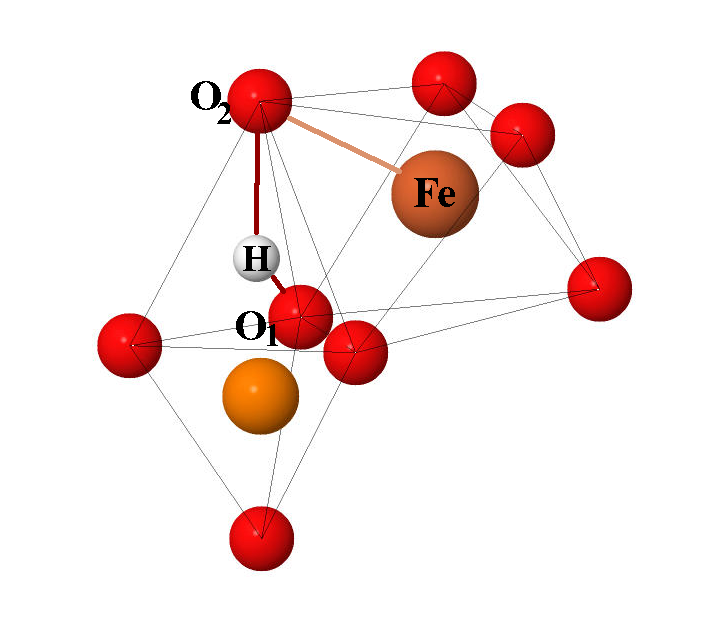
\includegraphics[width=0.9\linewidth]{pictures/tet1beforeCROP.png} \\ a)}
\end{minipage}
\hfill
\begin{minipage}[ht]{0.49\linewidth}
\center{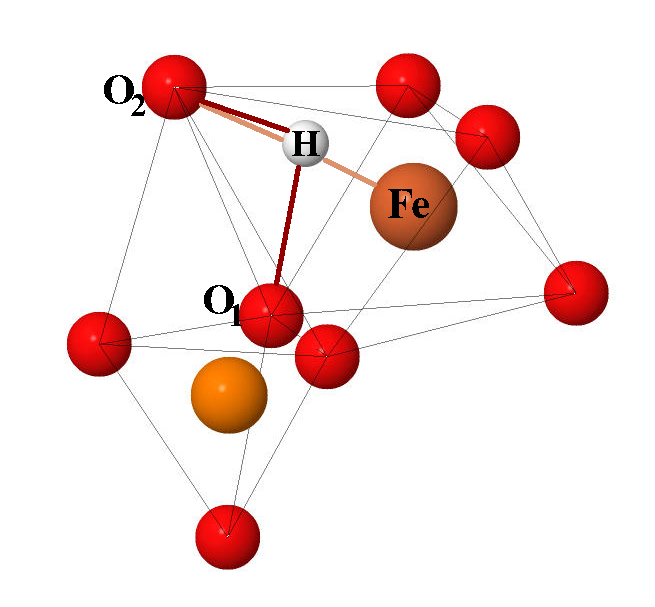
\includegraphics[width=0.9\linewidth]{pictures/tet1afterCROP.png} \\ b)}
\end{minipage}
\caption{Changes of hydrogen localization afret strucrural optimization in 1 case of tetrahedral void}
\label{ris:tet1}
\end{figure}

\begin{figure}[h]
\begin{minipage}[h]{0.49\linewidth}
\center{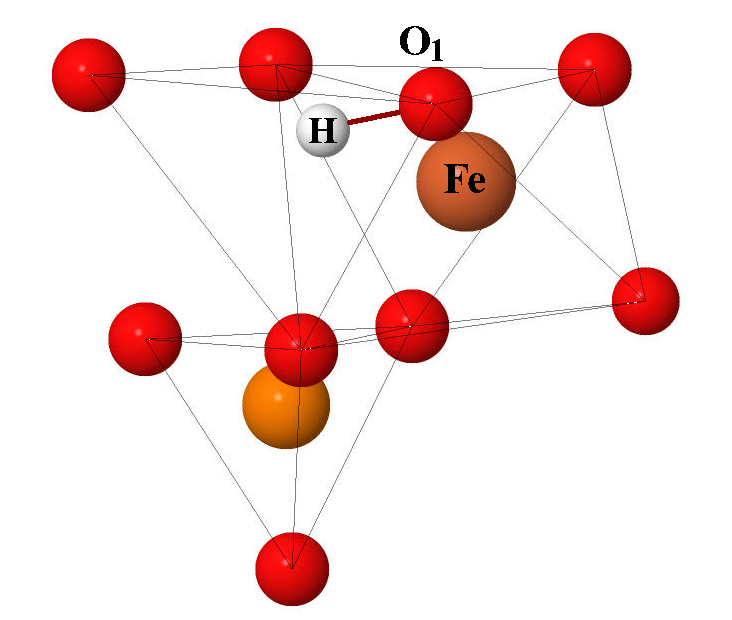
\includegraphics[width=0.9\linewidth]{pictures/tet2beforeCROP.png} \\ a)}
\end{minipage}
\hfill
\begin{minipage}[h]{0.49\linewidth}
\center{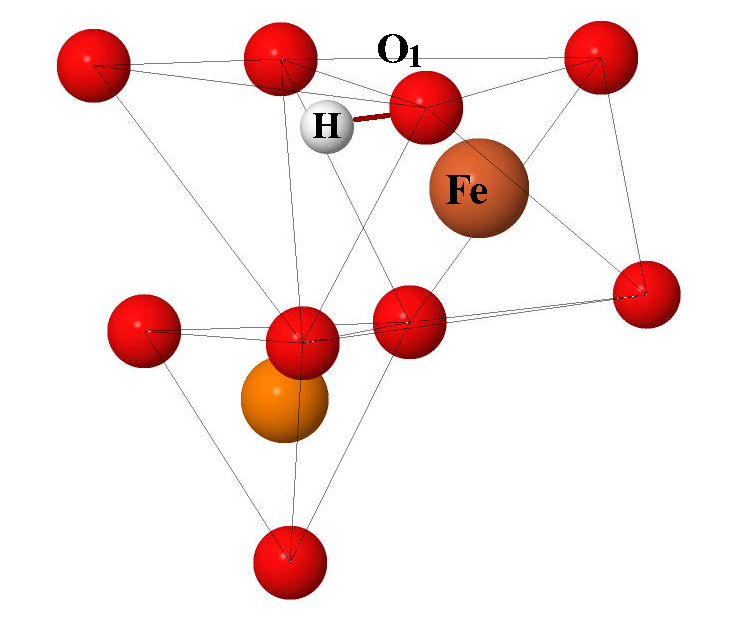
\includegraphics[width=0.9\linewidth]{pictures/tet2afterCROP.png} \\ b)}
\end{minipage}
\caption{Changes of hydrogen localization afret strucrural optimization in 2 case of tetrahedral void}
\label{ris:tet2}
\end{figure}

\textbf{3. Interstitial hydrogen in combination with lithium vacancy in LFP}

For each of possible configurations of interstitial hydrogen within pure LFP the situation with deintercalated lithium was considered. As example, the structure of LFP with interstitial hydrogen in first type of octahedral void site will be discussed below and the table of change in energy for possible configurations will be provided.

For LFP with hydrogen in place of octahedral void site in couple with lithium deintercalated atom the change of its localization are presented in Fig.\ref{ris:oct1-Li}. Distances between heighboring atoms were changed like: Fe-H from 1.99 \AA to 2.04 \AA; H-O$_1$ from 1.99 \AA to 1.02 \AA; H-O$_2$ from 1.55 \AA to 1.67 \AA. Generally, for all possible interstitial position the change of configuration of atoms and relative distanced have really small amount, and the energy of unit cell was changed slightly too. All of these results are provided in Table \ref{tabular:Liinter}.  

\begin{figure}[h]
\begin{minipage}[h]{0.49\linewidth}
\center{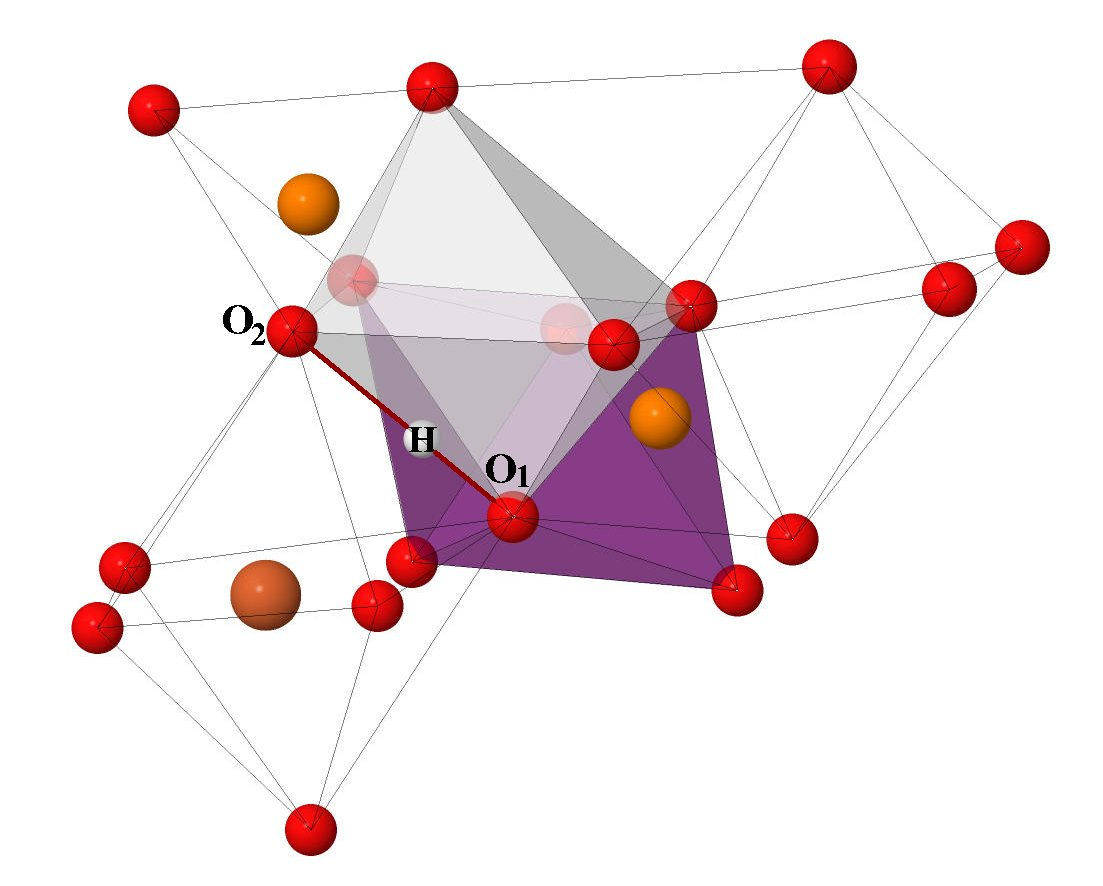
\includegraphics[width=0.9\linewidth]{pictures/oct1before-LiCROP.png} \\ a)}
\end{minipage}
\hfill
\begin{minipage}[h]{0.49\linewidth}
\center{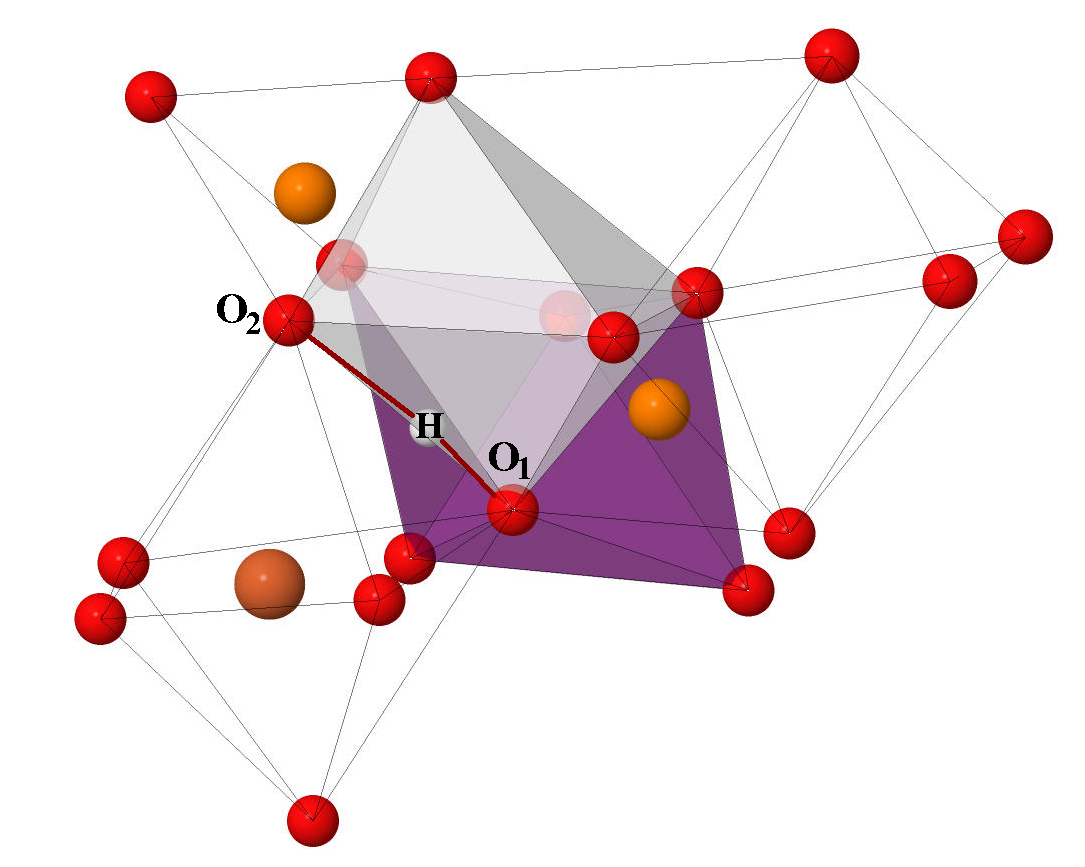
\includegraphics[width=0.9\linewidth]{pictures/oct1after-LiCROP.png} \\ b)}
\end{minipage}
\caption{Changes of hydrogen localization after strucrural optimization in 1 case of octahedral void with deintercalated lithium atom}
\label{ris:oct1-Li}
\end{figure}

\clearpage


%\caption{Characteristics of different defects}
\begin{adjustbox}{angle=90}
    %\begin{table}[h!]
    \centering
        %\centering
        \resizebox{18cm}{!}{
        \begin{tabular}{|c|c|c|c|c|c|c|c|}
            %& & & & & &\\
            \hline
            \textbf{Type} & \textbf{Neighborhood} & \textbf{Initial}& \textbf{Relax} & \textbf{Relax+Li$_{vac}$} & \textbf{E$_{form}$ of} & \textbf{E$_{form}$ +U} & \textbf{E$_{form}$ of } \\
            & & & & & \textbf{H$_{defect}$, eV} & & \textbf{H$_{defect}$+Li$_{vac}$, eV} \\
            \hline
            %& & & & & & \\
            Octahedral & H-Fe &  1.95 \AA &  1.99 \AA & 2.04 \AA  & -0.47 &  & -0.94 \\ 
            void 1 & H-O$_1$ & 0.99 \AA & 1.04 \AA & 1.02 \AA & & & \\
             & H-O$_2$ & 2.10 \AA & 1.55 \AA & 1.67 \AA & & & \\
            \hline
            %& & & & & &\\
            Octahedral& P-H & 1.16 \AA & 2.09 \AA & 2.19 \AA & -0.60 & & -0.94 \\
            void 2 & H-O$_1$ &  1.04 \AA & 1.01 \AA & 1.00 \AA & & &\\
            & H-O$_2$ & 2.52 \AA & 1.84 \AA& 2.07 \AA & & &\\
            \hline
            %& & & & & &\\
            Tetrahedral 1 & H-Fe & 2.09 \AA & 1.48 \AA & 1.47 \AA & -0.77 & & -0.7656 \\
            void  & H-O$_1$ & 1.84 \AA & 2.54 \AA & 2.53 \AA & & &\\
            & H-O$_2$ & 1.69 \AA & 1.54 \AA & 1.61 \AA & & & \\
            \hline
            %& & & & & & \\
            Tetrahedral 2 & H-O$_1$ & 1.2 \AA & 0.99 \AA & 1.00 \AA & -0.67 & & -1.10 \\
            %void 2 &  & & & & & & \\
            \hline
            %& & & & & & \\
            Substitutional &  &  &  &  & a) -1.89 eV & a) –0.34 eV & - \\
            hydrogen in place of  & H-O$_1$ & 0.99 \AA & 1.00 \AA & - & b) -3.05 eV & b) 0.89 eV & - \\
            lithium vacancy  &  & & & & & & \\
            \hline
            %& & & & & & & \\
            Substitutional & H$_1$-O$_1$ & 1.25 \AA & 1.00 \AA & - & a) -0.508 & & - \\
            2 hydrogens in place of  & H$_1$-O$_3$ & 2.71 \AA & - & & b) -2.93 eV & b) 0.88 eV & -\\
            iron vacancy  & H$_2$-O$_2$ & 1.20 \AA & 0.99 \AA & - & & &- \\
            & H$_2$-O$_3$ & 2.00 \AA & 1.94 \AA & - & & & -\\
            \hline
            %& & & & & & & \\
            4 hydrogen & (O-H)$_{1}$ &  & 0.97 \AA &  & a) -3.3307 & & - \\ 
            in P vacancy & (O-H)$_{2}$ & & 1.00 \AA& & b) -2.88 eV & b) 0.53 eV & - \\
            site  & (O-H)$_{3}$ & & 1.00 \AA & & & & \\
            & (O-H)$_{4}$ & & 0.98 \AA & & & & \\
            \hline
            %& & & & & & & \\
            5 hydrogen & (O-H)$_{1}$ & &  0.98 \AA &  & a) -2.8486 & & -\\ 
            in P vacancy & (O-H)$_{2}$ & & 1.01 \AA & &b) -2.49 eV &b) 0.73 eV & -\\
            site  & (O-H)$_{3}$ & & 1.01 \AA & & & & \\
            & (O-H)$_{4}$ & & 0.97 \AA & & & & \\
            & (O-H)$_{5}$ & & 1.04 \AA & & & & \\
            \hline
            \label{tabular:Liinter}
        \end{tabular}}
    %\caption{Characteristics of different defects}
    %\end{table}
\end{adjustbox}



\newpage

\textbf{4. Substitutional hydrogen in place of lithium vacancy within LFP}

The possible configuration of substitutional hydrogen in place of lithium vacancy was observed. In this case the change of localization of hydrogen and relative distences are shown in picture below: during relaxation of atomic structure the distance between hydrogen and neighbooring oxygen H-O$_1$ have been changing from 0.99 \AA to 1.00 \AA, Fig.\ref{ris:Li1H}. The corresponding formation energy of such substitutional defect is equal to -1.8864 eV.

\begin{figure}[h]
\begin{minipage}[h]{0.49\linewidth}
\center{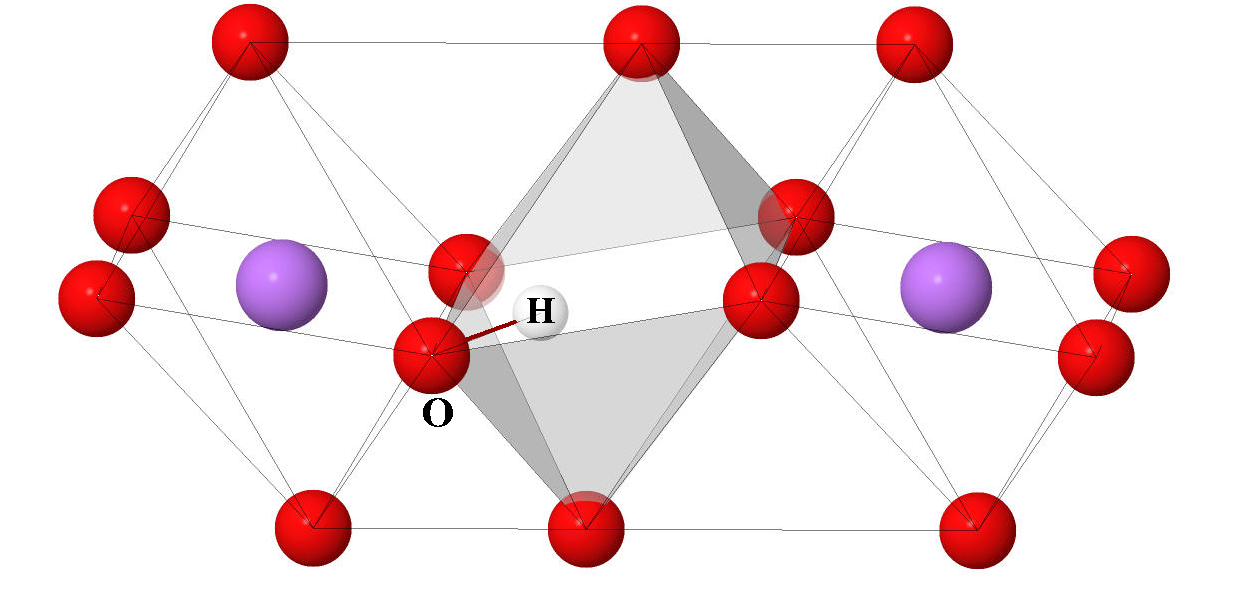
\includegraphics[width=0.9\linewidth]{pictures/Li1HbeforeCROP.png} \\ a)}
\end{minipage}
\hfill
\begin{minipage}[h]{0.49\linewidth}
\center{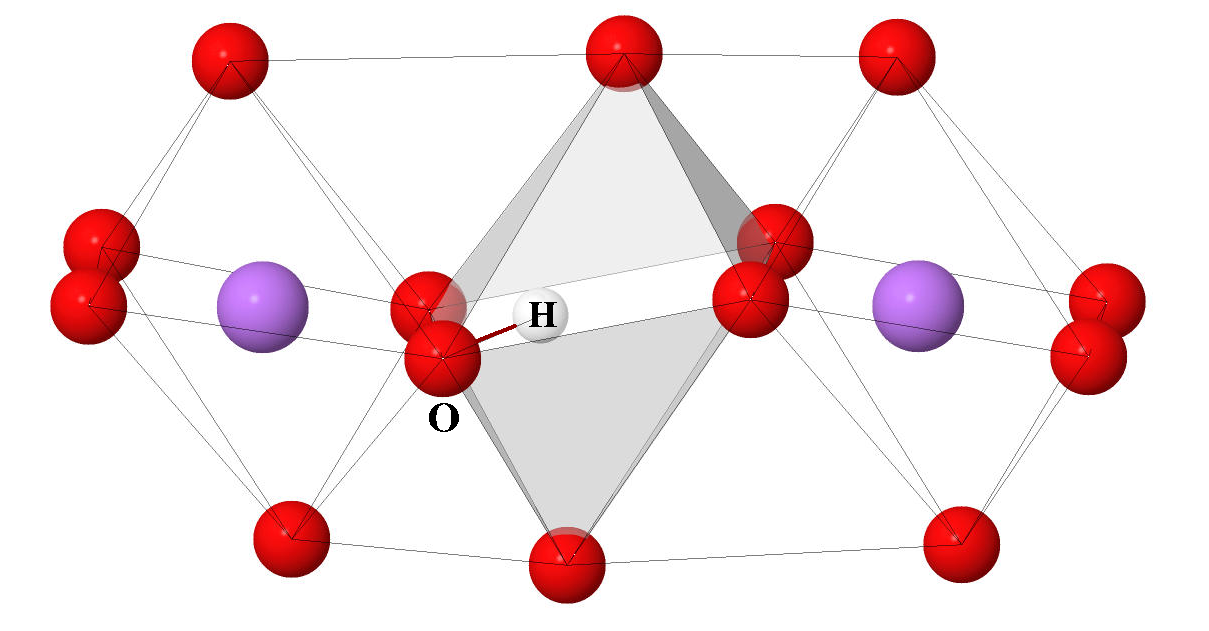
\includegraphics[width=0.9\linewidth]{pictures/Li1HafterCROP.png} \\ b)}
\end{minipage}
\caption{Changes of substitutional hydrogen in place of lithium vacancy after strucrural optimization}
\label{ris:Li1H}
\end{figure}

\textbf{5. Substitutional hydrogen in place of iron vacancy within LFP}

The next substitutional defect is hydrogen in place of iron atom. According to the valency of the last, two of hydrogen can be placed in the structure with one iron atom absence in order to achieve charging neutrality. The distinction in distance between neighbooring atoms is presented in the Fig.\ref{ris:Fe2H}. In this case distances between first hydrogen and oxygen H$_1$-O$_1$ is changes from 1.25 \AA to 1.00 \AA; H$_1$-O$_3$ - frrom 2.71 \AA to 2.00 \AA. Distanses between second hydrogen and neighbooring oxygens are changed like: H$_2$-O$_2$ from 1.20 \AA to 0.99 \AA, H$_2$-O$_3$ from 2.27 \AA to 1.94 \AA. The formation energy of such type of substitutional defect is equal to -0.5079 eV.


\begin{figure}[h]
\begin{minipage}[h]{0.49\linewidth}
\center{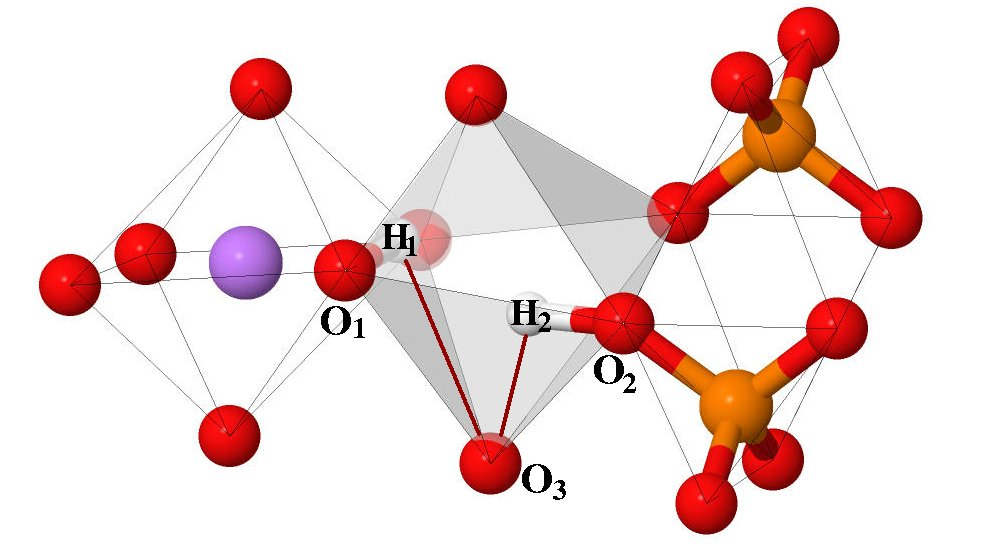
\includegraphics[width=0.9\linewidth]{pictures/Fe2HbeforeCROP.png} \\ a)}
\end{minipage}
\hfill
\begin{minipage}[h]{0.49\linewidth}
\center{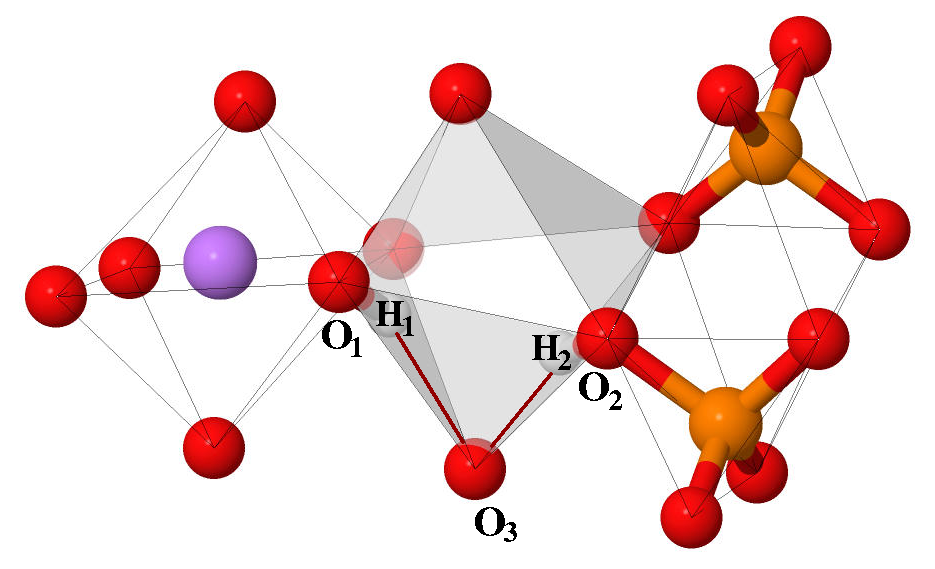
\includegraphics[width=0.9\linewidth]{pictures/Fe2HafterCROP.png} \\ b)}
\end{minipage}
\caption{Changes of substitutional hydrogen in place of iron atom vacancy after strucrural optimization}
\label{ris:Fe2H}
\end{figure}

\textbf{6. Substitutional hydrogen in place of phosphorus vacancy within LFP}

The last possible substitutional hydrogen defect is its localization in place of phosphorus vacancy site. If one phosphorus atom are removed from its stable position, five of iron atoms in neighboring area are changed their oxidation state from 2+ to 3+. There can be two scenario of substitutional defects: four or five hydrogen atoms in place of phosphorus vacancy. For atoms of hydrogen can build OH bonds with each of oxygen in tetrahedral environment. In this case just one iron atom have changed its oxidation state. According to achieve charging neutrality and taking into accaunt the valency of phosphorus atom within crystal P$^{5+}$ there are need to use 5 atoms of hydrogen. In this case all iron atoms exist in their oxidation state is equal to 2+ without changing. But, according to energy characteristics, the last situation is less likely, Table \ref{tabular:4or5H}. 

Some small changes of atom positions have been happening in the structure during the relaxation calculation. The comparison between two possible substitutional defects are presented in the Fig.\ref{ris:P45H}.For LFP with phosphorus vacancy and four hydrogen atoms as an impuritythe distances between hydrogen and neighboring oxygen are: (O-H)$_{1}$ = 0.97 \AA, (O-H)$_{2}$ = 1.00 \AA, (O-H)$_{3}$ = 1.00 \AA, (O-H)$_{4}$ = 0.98 \AA. In case of five substitutional hydrogen: (O-H)$_{1}$ = 0.98 \AA, (O-H)$_{2}$ = 1.01 \AA, (O-H)$_{3}$ = 1.01 \AA, (O-H)$_{4}$ = 0.97 \AA, (O-H)$_{5}$ = 1.04 \AA.


\begin{figure}[h]
\begin{minipage}[h]{0.49\linewidth}
\center{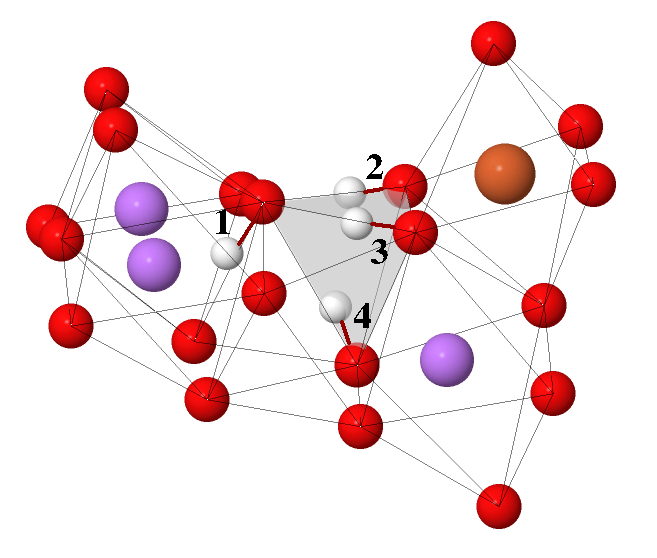
\includegraphics[width=0.9\linewidth]{pictures/P4HafterCROP.png} \\ a)P vacancy with 4 H}
\end{minipage}
\hfill
\begin{minipage}[h]{0.49\linewidth}
\center{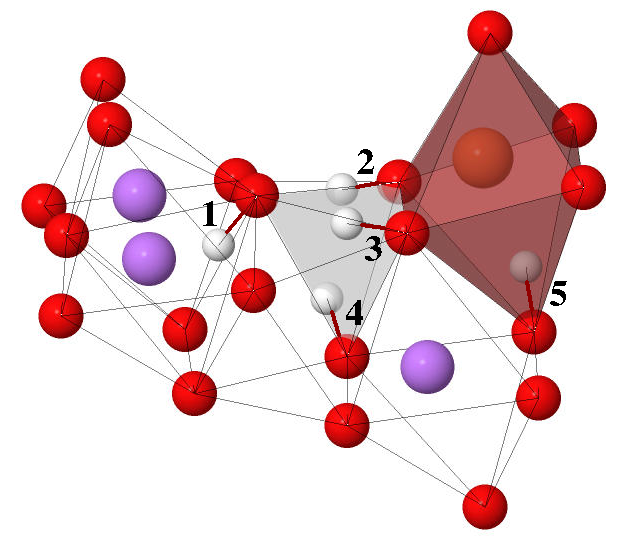
\includegraphics[width=0.9\linewidth]{pictures/P5HafterCROP.png} \\ b) P vacancy with 5 H}
\end{minipage}
\caption{Substitutional hydrogen in place of P atom vacancy after strucrural optimization}
\label{ris:P45H}
\end{figure}



\begin{table}[h]
\caption{Characteristics of P/4H and P/5H defects}
\label{tabular:4or5H}
\begin{center}
\begin{tabular}{|c|c|c|c|}
\hline
& & & \\
\textbf{Type} & \textbf{Bonds} & \textbf{Distance} & \textbf{E$_{form}$, eV} \\
\hline
& & & \\
4 hydrogen & (O-H)$_{1}$ &  0.97 \AA &  -3.3307 \\ 
in P vacancy & (O-H)$_{2}$ & 1.00 \AA & \\
site  & (O-H)$_{3}$ & 1.00 \AA & \\
& (O-H)$_{4}$ & 0.98 \AA &\\
\hline
& & & \\
5 hydrogen & (O-H)$_{1}$ &  0.98 \AA &  -2.8486 \\ 
in P vacancy & (O-H)$_{2}$ & 1.01 \AA & \\
site  & (O-H)$_{3}$ & 1.01 \AA & \\
& (O-H)$_{4}$ & 0.97 \AA & \\
& (O-H)$_{5}$ & 1.04 \AA & \\
\hline
\end{tabular}
\end{center}
\end{table}

1. 4H
2. 5H 